\flushbottom




%%============================================================================
%%============================================================================
\chapter{Conformal Mapping}




%% CONTINUE: write me



\raggedbottom
%%=============================================================================
\exercises{
\pagebreak
\flushbottom
\section{Exercises}








\begin{Exercise}
  Use an appropriate conformal map to find a non-trivial solution to 
  Laplace's equation 
  \[ 
  u_{x x}+u_{y y} = 0,
  \]
  on the wedge bounded by the $x$-axis and the line $y = x$ with boundary 
  conditions:
  \begin{enumerate}
  \item 
    $u=0$ on both sides.  
  \item 
    $\displaystyle \frac{\dd u}{\dd n} = 0$ on both sides (where $\mathbf{n}$ 
    is the inward normal to the boundary).
  \end{enumerate}
\end{Exercise}








\begin{Exercise}
  Consider
  \[ 
  u_{x x} + u_{y y} = \delta(x-\xi) \delta(y-\psi),
  \]
  on the quarter plane $x,y > 0$ with $u(x,0) = u(0,y) = 0$ (and $\xi,\psi > 0$). 
  \begin{enumerate}
  \item 
    Use image sources to find $u(x,y;\xi,\psi)$.
  \item 
    Compare this to the solution which would be obtained using
    conformal maps and the Green function for the upper half plane. 
  \item 
    Finally use this idea and conformal mapping to 
    discover how image sources are arrayed
    when the domain is now the wedge bounded by the $x$-axis and the line 
    $y = x$ (with $u = 0$ on both sides).
  \end{enumerate}
\end{Exercise}








\begin{Exercise}
  $\zeta = \xi + \imath \eta$ is an analytic function of $z$, $\zeta = \zeta(z)$.
  We assume that $\zeta'(z)$ is nonzero on the domain of interest.
  $u(x, y)$ is an arbitrary smooth function of $x$ and $y$.  
  When expressed in terms of $\xi$ and $\eta$, $u(x, y) = \upsilon(\xi, \eta)$.  
  In Exercise~\ref{exercise w=u+iv is analytic} we showed that
  \[
  \frac{\partial^2 \upsilon}{\partial \xi^2} + \frac{\partial^2 \upsilon}{\partial \eta^2} =
  \left| \frac{\dd \zeta}{\dd z} \right|^{-2}
  \left( \frac{\partial^2 u}{\partial x^2} + \frac{\partial^2 u}{\partial y^2} \right).
  \]
  \begin{enumerate}
  \item
    Show that if $u$ satisfies Laplace's equation in the $z$-plane, 
    \[
    u_{x x} + u_{y y} = 0,
    \]
    then $\upsilon$ satisfies Laplace's equation in the $\zeta$-plane,
    \[
    \upsilon_{\xi \xi} + \upsilon_{\eta \eta} = 0,
    \]
  \item
    Show that if $u$ satisfies Helmholtz's equation in the $z$-plane, 
    \[
    u_{x x} + u_{y y} = \lambda u,
    \]
    then in the $\zeta$-plane $\upsilon$ satisfies
    \[
    \upsilon_{\xi \xi} + \upsilon_{\eta \eta} = \lambda \left| \frac{\dd z}{\dd \zeta} \right|^2 \upsilon.
    \]
  \item
    Show that if $u$ satisfies Poisson's equation in the $z$-plane, 
    \[
    u_{x x} + u_{y y} = f(x,y),
    \]
    then $\upsilon$ satisfies Poisson's equation in the $\zeta$-plane,
    \[
    \upsilon_{\xi \xi} + \upsilon_{\eta \eta} = \left| \frac{\dd z}{\dd \zeta} \right|^2 \phi(\xi,\eta),
    \]
    where $\phi(\xi,\eta) = f(x,y)$.
  \item
    Show that if in the $z$-plane, $u$ satisfies the Green function problem,
    \[
    u_{x x} + u_{y y} = \delta(x-x_0) \delta(y-y_0),
    \]
    then in the $\zeta$-plane, $\upsilon$ satisfies the Green function problem,
    \[
    \upsilon_{\xi \xi} + \upsilon_{\eta \eta} = \delta(\xi-\xi_0) \delta(\eta-\eta_0).
    \]
  \end{enumerate}
\end{Exercise}









%% semi-circular rod
\begin{Exercise}
  A semi-circular rod of infinite extent is maintained at temperature
  $T = 0$ on the flat side and at $T = 1$ on the curved surface:
  \[
  x^2 + y^2 = 1, \quad y > 0.
  \]
  Use the conformal mapping
  \[
  w = \xi + \imath \eta = \frac{1+z}{1-z}, \quad z = x + \imath y,
  \]
  to formulate the problem in terms of $\xi$ and $\eta$.  Solve the 
  problem in terms of these variables.
  This problem is solved with an eigenfunction expansion in
  Exercise~\ref{exercise potential semi-circular rod}.  
  Verify that the two solutions agree.
\end{Exercise}



%% Laplace's equation, infinite strip, mixed boundary conditions.
\begin{Exercise}
  Consider Laplace's equation on the domain $-\infty < x < \infty$, 
  $0 < y < \pi$, subject to the mixed boundary conditions,
  \begin{alignat*}{2}
    &u = 1 &\quad &\mathrm{on}\ y = 0,\ x > 0, \\
    &u = 0 &\quad &\mathrm{on}\ y = \pi,\ x > 0, \\
    &u_y = 0 &\quad &\mathrm{on}\ y = 0,\ y = \pi,\ x < 0.
  \end{alignat*}
  Because of the mixed boundary conditions, ($u$ and $u_y$ are given on separate
  parts of the same boundary), this problem cannot be solved with separation 
  of variables.  Verify that the conformal map,
  \[
  \zeta = \cosh^{-1}( \e^z ),
  \]
  with $z = x + \imath y$, $\zeta = \xi + \imath \eta$ maps the infinite interval into
  the semi-infinite interval, $\xi > 0$, $0 < \eta < \pi$.  Solve Laplace's
  equation with the appropriate boundary conditions in the $\zeta$ plane by
  inspection.  Write the solution $u$ in terms of $x$ and $y$.
\end{Exercise}












\raggedbottom
}
%%=============================================================================
\hints{
\pagebreak
\flushbottom
\section{Hints}




\begin{Hint}
  %% CONTINUE
\end{Hint}







\begin{Hint}
  %% CONTINUE
\end{Hint}




\begin{Hint}
  %% CONTINUE
\end{Hint}




%% semi-circular rod
\begin{Hint}
  Show that $w = (1+z)/(1-z)$ maps the semi-disc, $0 < r < 1$, 
  $0 < \theta < \pi$ to the first quadrant of the $w$ plane.  Solve the 
  problem for $v(\xi,\eta)$ by taking Fourier sine transforms in $\xi$ 
  and $\eta$.  

  To show that the solution for $v(\xi,\eta)$ is equivalent to the series
  expression for $u(r,\theta)$, first find an analytic function $g(w)$ 
  of which $v(\xi,\eta)$ is the imaginary part.  Change variables to 
  $z$ to obtain the analytic function $f(z) = g(w)$.  Expand $f(z)$ in 
  a Taylor series and take the imaginary part to show the equivalence
  of the solutions.
\end{Hint}



%% Laplace's equation, infinite strip, mixed boundary conditions.
\begin{Hint}
  To see how the boundary is mapped, consider the map,
  \[
  z = \log ( \cosh \zeta ).
  \]
  The problem in the $\zeta$ plane is,
  \begin{gather*}
    v_{\xi\xi} + v_{\eta\eta} = 0, \quad \xi > 0, \quad 0 < \eta < \pi, \\
    v_\xi(0, \eta) = 0, \quad v(\xi, 0) = 1, \quad v(\xi, \pi) = 0.
  \end{gather*}
  To solve this, find a plane that satisfies the boundary conditions.
\end{Hint}












\raggedbottom
}
{
}
%%=============================================================================
\solutions{
\pagebreak
\flushbottom
\section{Solutions}






\begin{Solution}
  We map the wedge to the upper half plane with the conformal transformation
  $\zeta = z^4$.
  \begin{enumerate}
  \item 
    We map the wedge to the upper half plane with the conformal transformation
    $\zeta = z^4$.  The new problem is
    \[
    u_{\xi \xi} + u_{\eta \eta} = 0, \quad u(\xi,0) = 0.
    \]
    This has the solution $u = \eta$.  We transform this problem back to the wedge.
    \begin{gather*}
      u(x,y) = \Im \left( z^4 \right)
      \\
      u(x,y) = \Im \left( x^4 + \imath 4 x^3 y - 6 x^2 y^2 - \imath 4 x y^3 + y^4 \right)
      \\
      u(x,y) = 4 x^3 y - 4 x y^3 
      \\
      \boxed{
        u(x,y) = 4 x y \left( x^2 - y^2 \right)
        }
    \end{gather*}
  \item
    We don't need to use conformal mapping to solve the problem with Neumman
    boundary conditions.  $u = c$ is a solution to 
    \[
    u_{x x} + u_{y y} = 0, \quad \frac{\dd u}{\dd n} = 0
    \]
    on any domain.
  \end{enumerate}
\end{Solution}









\begin{Solution}
  \begin{enumerate}
  \item 
    We add image sources to satisfy the boundary conditions.
    \[
    u_{x x}+u_{y y} = \delta(x-\xi) \delta(y-\eta) -  \delta(x+\xi) \delta(y-\eta) - \delta(x-\xi) \delta(y+\eta) + \delta(x+\xi) \delta(y+\eta)
    \]
    \begin{multline*}
      u = \frac{1}{2 \pi} \left( \ln \left( \sqrt{ (x-\xi)^2 + (y-\eta)^2 } \right)
        - \ln \left( \sqrt{ (x+\xi)^2 + (y-\eta)^2 } \right) \right.
      \\
      \left. - \ln \left( \sqrt{ (x-\xi)^2 + (y+\eta)^2 } \right)
        + \ln \left( \sqrt{ (x+\xi)^2 + (y+\eta)^2 } \right) \right)
    \end{multline*}
    \[
    \boxed{
      u = \frac{1}{4 \pi} \ln \left( 
        \frac{ \left((x-\xi)^2 + (y-\eta)^2 \right) \left((x+\xi)^2 + (y+\eta)^2 \right) }
        { \left((x+\xi)^2 + (y-\eta)^2 \right) \left((x-\xi)^2 + (y+\eta)^2 \right) }
      \right)
      }
    \]
  \item 
    The Green function for the upper half plane is
    \[
    G = \frac{1}{4 \pi} \ln \left( 
      \frac{ \left((x-\xi)^2 + (y-\eta)^2 \right) }{ \left((x-\xi)^2 + (y+\eta)^2 \right) }
    \right)
    \]
    We use the conformal map, 
    \begin{gather*}
      c = z^2, \quad c = a + \imath b.
      \\
      a = x^2 - y^2, \quad b = 2 x y
    \end{gather*}
    We compute the Jacobian of the mapping.
    \[
    J = 
    \begin{vmatrix}
      a_x & a_y \\
      b_x & b_y
    \end{vmatrix}
    = 
    \begin{vmatrix}
      2 x & - 2 y \\
      2 y & 2 x
    \end{vmatrix}
    =
    4 \left( x^2 + y^2 \right)
    \]
    We transform the problem to the upper half plane, solve the problem there, 
    and then transform back to the first quadrant.
    \begin{gather*}
      u_{x x} + u_{y y} = \delta(x-\xi) \delta(y-\eta)
      \\
      \left( u_{a a} + u_{b b} \right) \left| \frac{\dd c}{\dd z} \right|^2 
      = 4 \left( x^2 + y^2 \right) \delta(a - \alpha) \delta(b - \beta)
      \\
      \left( u_{a a} + u_{b b} \right) \left| 2 z \right|^2 
      = 4 \left( x^2 + y^2 \right) \delta(a - \alpha) \delta(b - \beta)
      \\
      u_{a a} + u_{b b} = \delta(a - \alpha) \delta(b - \beta)
      \\
      u = \frac{1}{4 \pi} \ln \left( 
        \frac{ \left((a-\alpha)^2 + (b-\beta)^2 \right) }{ \left((a-\alpha)^2 + (b+\beta)^2 \right) }
      \right)
      \\
      u = \frac{1}{4 \pi} \ln \left( 
        \frac{ \left((x^2 - y^2 - \xi^2 + \eta^2)^2 + (2 x y - 2 \xi \eta)^2 \right) }
        { \left((x^2 - y^2 - \xi^2 + \eta^2)^2 + (2 x y + 2 \xi \eta)^2 \right) }
      \right)
      \\
      \boxed{
        u = \frac{1}{4 \pi} \ln \left( 
          \frac{ \left((x-\xi)^2 + (y-\eta)^2 \right) \left((x+\xi)^2 + (y+\eta)^2 \right) }
          { \left((x+\xi)^2 + (y-\eta)^2 \right) \left((x-\xi)^2 + (y+\eta)^2 \right) }
        \right)
        }
    \end{gather*}
    We obtain the some solution as before.
  \item 
    First consider
    \[
    \Delta u = \delta(x-\xi) \delta(y-\eta), \quad u(x,0) = u(x,x) = 0.
    \]
    Enforcing the boundary conditions will require 7 image sources obtained 
    from 4 odd reflections.  Refer to Figure~\ref{sector_delta} to see the 
    reflections pictorially.
    First we do a negative reflection across the line $y = x$, which adds 
    a negative image source at the point $(\eta,\xi)$ This enforces the 
    boundary condition along $y = x$.
    \[
    \Delta u = \delta(x-\xi) \delta(y-\eta) - \delta(x-\eta) \delta(y-\xi), \quad u(x,0) = u(x,x) = 0
    \]
    Now we take the negative image of the reflection of these two sources across
    the line $y = 0$ to enforce the boundary condition there.
    \[
    \Delta u = \delta(x-\xi) \delta(y-\eta) - \delta(x-\eta) \delta(y-\xi) - \delta(x-\xi) \delta(y+\eta) + \delta(x-\eta) \delta(y+\xi)
    \]
    The point sources are no longer odd symmetric about $y = x$.  We add two 
    more image sources to enforce that boundary condition.
    \begin{multline*}
      \Delta u = \delta(x-\xi) \delta(y-\eta) - \delta(x-\eta) \delta(y-\xi) - \delta(x-\xi) \delta(y+\eta) + \delta(x-\eta) \delta(y+\xi)
      \\
      + \delta(x+\eta) \delta(y-\xi) - \delta(x+\xi) \delta(y-\eta)
    \end{multline*}
    Now sources are no longer odd symmetric about $y = 0$.  Finally we add 
    two more image sources to enforce that boundary condition.  Now the sources
    are odd symmetric about both $y = x$ and $y = 0$.
    \begin{multline*}
      \Delta u = \delta(x-\xi) \delta(y-\eta) - \delta(x-\eta) \delta(y-\xi) - \delta(x-\xi) \delta(y+\eta) + \delta(x-\eta) \delta(y+\xi)
      \\
      + \delta(x+\eta) \delta(y-\xi) - \delta(x+\xi) \delta(y-\eta) + \delta(x+\xi) \delta(y+\eta) - \delta(x+\eta) \delta(y+\xi) 
    \end{multline*}
    \begin{figure}[h!]
      \begin{center}
        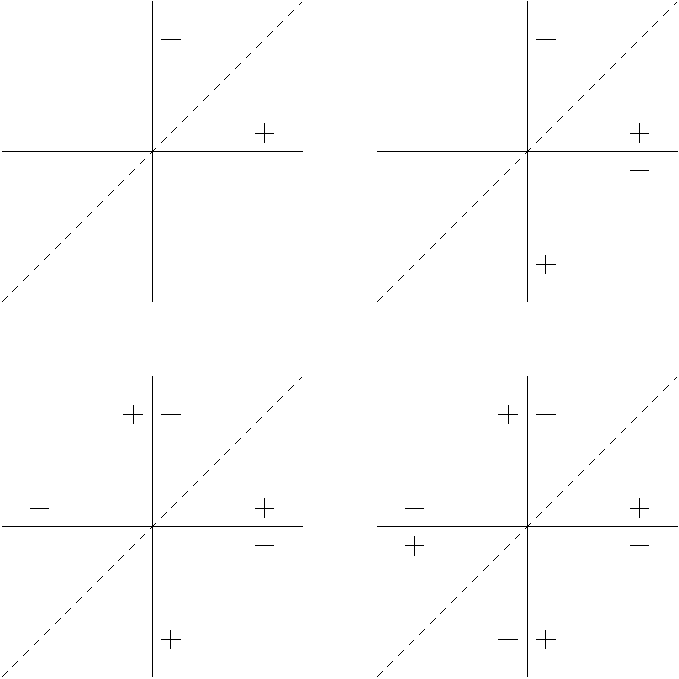
\includegraphics[width=0.5\textwidth]{pde/conformal/sector_delta}
      \end{center}
      \caption{Odd reflections to enforce the boundary conditions.}
      \label{sector_delta}
    \end{figure}
  \end{enumerate}
\end{Solution}










\begin{Solution}
  \[
  \frac{\partial^2 \upsilon}{\partial \xi^2} + \frac{\partial^2 \upsilon}{\partial \eta^2} =
  \left| \frac{\dd \zeta}{\dd z} \right|^{-2}
  \left( \frac{\partial^2 u}{\partial x^2} + \frac{\partial^2 u}{\partial y^2} \right).
  \]
  \begin{enumerate}
  \item
    \begin{gather*}
      u_{x x} + u_{y y} = 0
      \\
      \left| \frac{\dd \zeta}{\dd z} \right|^2 \left( \upsilon_{\xi \xi} + \upsilon_{\eta \eta} \right) = 0
      \\
      \upsilon_{\xi \xi} + \upsilon_{\eta \eta} = 0
    \end{gather*}
  \item
    \begin{gather*}
      u_{x x} + u_{y y} = \lambda u
      \\
      \left| \frac{\dd \zeta}{\dd z} \right|^2 \left( \upsilon_{\xi \xi} + \upsilon_{\eta \eta} \right) = \lambda \upsilon
      \\
      \upsilon_{\xi \xi} + \upsilon_{\eta \eta} = \lambda \left| \frac{\dd z}{\dd \zeta} \right|^2 \upsilon
    \end{gather*}
  \item
    \begin{gather*}
      u_{x x} + u_{y y} = f(x,y)
      \\
      \left| \frac{\dd \zeta}{\dd z} \right|^2 \left( \upsilon_{\xi \xi} + \upsilon_{\eta \eta} \right) = \phi(\xi,\eta)
      \\
      \upsilon_{\xi \xi} + \upsilon_{\eta \eta} = \left| \frac{\dd z}{\dd \zeta} \right|^2 \phi(\xi,\eta)
    \end{gather*}
  \item
    The Jacobian of the mapping is
    \[
    J = 
    \begin{vmatrix}
      x_\xi & y_\xi \\
      x_\eta & y_\eta
    \end{vmatrix}
    = x_\xi y_\eta - x_\eta y_\xi
    = x_\xi^2 + y_\xi^2.
    \]
    Thus the Dirac delta function on the right side gets mapped to
    \[
    \frac{1}{x_\xi^2 + y_\xi^2} \delta(\xi-\xi_0) \delta(\eta-\eta_0).
    \]
    Next we show that $\left| \dd z / \dd \zeta \right|^2$ has the same value as 
    the Jacobian.
    \[
    \left| \frac{\dd z}{\dd \zeta} \right|^2
    = (x_\xi + \imath y_\xi)(x_\xi - \imath y_\xi) 
    = x_\xi^2 + y_\xi^2
    \]
    Now we transform the Green function problem.
    \begin{gather*}
      u_{x x} + u_{y y} = \delta(x-x_0) \delta(y-y_0)
      \\
      \left| \frac{\dd \zeta}{\dd z} \right|^2 \left( \upsilon_{\xi \xi} + \upsilon_{\eta \eta} \right)
      = \frac{1}{x_\xi^2 + y_\xi^2} \delta(\xi-\xi_0) \delta(\eta-\eta_0)
      \\
      \upsilon_{\xi \xi} + \upsilon_{\eta \eta} = \delta(\xi-\xi_0) \delta(\eta-\eta_0)
    \end{gather*}
  \end{enumerate}
\end{Solution}







%% semi-circular rod
\begin{Solution}
  The mapping,
  \[
  w = \frac{1+z}{1-z},
  \]
  maps the unit semi-disc to the first quadrant of the complex plane.

  We write the mapping in terms of $r$ and $\theta$.
  \[
  \xi + \imath \eta = \frac{1 + r \e^{\imath \theta}}{1 - r \e^{\imath \theta}}
  = \frac{ 1 - r^2 + \imath 2 r \sin \theta }{ 1 + r^2 - 2 r \cos \theta }
  \]
  \begin{align*}
    \xi &= \frac{ 1 - r^2 }{ 1 + r^2 - 2 r \cos \theta } \\
    \eta &= \frac{ 2 r \sin \theta }{ 1 + r^2 - 2 r \cos \theta }
  \end{align*}
  Consider a semi-circle of radius $r$.  The image of this under the 
  conformal mapping is a semi-circle of radius $\frac{2r}{1-r^2}$ and center
  $\frac{1+r^2}{1-r^2}$ in the first quadrant of the $w$ plane.  This 
  semi-circle intersects the $\xi$ axis at $\frac{1-r}{1+r}$ and 
  $\frac{1+r}{1-r}$.   As $r$ ranges from zero to one, these semi-circles
  cover the first quadrant of the $w$ plane.
  (See Figure~\ref{cm_sc2fq}.)

  \begin{figure}[h!]
    \begin{center}
      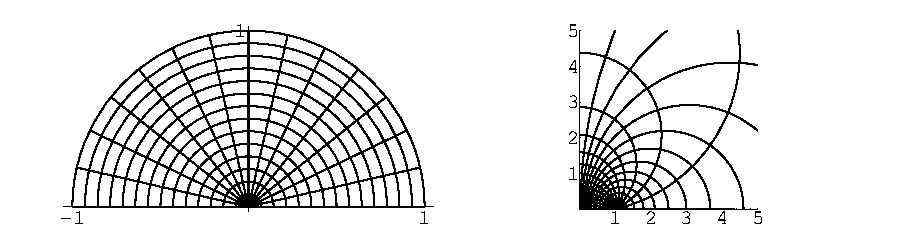
\includegraphics[width=\textwidth]{pde/conformal/cm_sc2fq}
    \end{center}
    \caption{The conformal map.}
    \label{cm_sc2fq}
  \end{figure}

  We also note how the boundary of the semi-disc is mapped to the 
  boundary of the first quadrant of the $w$ plane.  The line segment
  $\theta = 0$ is mapped to the real axis $\xi > 1$.  The line segment
  $\theta = \pi$ is mapped to the real axis $0 < \xi < 1$.  Finally,
  the semi-circle $r = 1$ is mapped to the positive imaginary axis.

  The problem for $v(\xi,\eta)$ is,
  \begin{gather*}
    v_{\xi\xi} + v_{\eta\eta} = 0, \quad \xi > 0, \quad \eta > 0, \\
    v(\xi,0) = 0, \quad v(0,\eta) = 1.
  \end{gather*}
  We will solve this problem with the Fourier sine transform.  We take the
  Fourier sine transform of the partial differential equation, first
  in $\xi$ and then in $\eta$.
  \begin{gather*}
    -\alpha^2 \hat{v}(\alpha, \eta) + \frac{\alpha}{\pi} v(0, \eta) 
    + \hat{v}(\alpha,\eta) = 0, \quad \hat{v}(\alpha, 0) = 0 \\
    -\alpha^2 \hat{v}(\alpha, \eta) + \frac{\alpha}{\pi} 
    + \hat{v}(\alpha,\eta) = 0, \quad \hat{v}(\alpha, 0) = 0 \\
    -\alpha^2 \hat{\hat{v}}(\alpha, \beta) + \frac{\alpha}{\pi^2 \beta} 
    - \beta^2 \hat{\hat{v}}(\alpha,\beta) 
    + \frac{\beta}{\pi} \hat{v}(\alpha, 0) = 0 \\
    \hat{\hat{v}}(\alpha, \beta) = \frac{\alpha}{\pi^2 \beta (\alpha^2 + \beta^2)}
  \end{gather*}
  Now we utilize the Fourier sine transform pair,
  \[
  \mathcal{F}_s \left[ \e^{-c x} \right] = \frac{\omega / \pi}{ \omega^2 + c^2},
  \]
  to take the inverse sine transform in $\alpha$.
  \[
  \hat{v}(\xi,\beta) = \frac{1}{\pi \beta} \e^{- \beta \xi}
  \]
  With the Fourier sine transform pair,
  \[
  \mathcal{F}_s \left[ 2 \arctan \left( \frac{x}{c} \right) \right] = 
  \frac{1}{\omega} \e^{-c \omega},
  \]
  we take the inverse sine transform in $\beta$ to obtain the solution.
  \[
  \boxed{
    v(\xi,\eta) = \frac{2}{\pi} \arctan \left( \frac{\eta}{\xi} \right)
    }
  \]
  Since $v$ is harmonic, it is the imaginary part of an analytic function
  $g(w)$.  By inspection, we see that this function is
  \[
  g(w) = \frac{2}{\pi} \log(w).
  \]
  We change variables to $z$, $f(z) = g(w)$.
  \[
  f(z) = \frac{2}{\pi} \log \left( \frac{1+z}{1-z} \right)
  \]
  We expand $f(z)$ in a Taylor series about $z = 0$,
  \[
  f(z) = \frac{4}{\pi} \sum_{\substack{n = 1 \\ \mathrm{odd}\ n}}^\infty
  \frac{z^n}{n},
  \]
  and write the result in terms of $r$ and $\theta$, $z = r \e^{\imath \theta}$.
  \[
  f(z) = \frac{4}{\pi} \sum_{\substack{n = 1 \\ \mathrm{odd}\ n}}^\infty
  \frac{r^n \e^{\imath \theta}}{n}
  \]
  $u(r,\theta)$ is the imaginary part of $f(z)$.
  \[
  \boxed{
    u(r,\theta) = \frac{4}{\pi} \sum_{\substack{n = 1 \\ \mathrm{odd}\ n}}^\infty
    \frac{1}{n} r^n \sin(n \theta)
    }
  \]
  This demonstrates that the solutions obtained with conformal mapping and 
  with an eigenfunction expansion in 
  Exercise~\ref{exercise potential semi-circular rod} agree.
\end{Solution}











%% Laplace's equation, infinite strip, mixed boundary conditions.
\begin{Solution}
  Instead of working with the conformal map from the $z$ plane to the $\zeta$
  plane,
  \[
  \zeta = \cosh^{-1} (\e^z),
  \]
  it will be more convenient to work with the inverse map,
  \[
  z = \log ( \cosh \zeta ),
  \]
  which maps the semi-infinite strip to the infinite one.  We determine how
  the boundary of the domain is mapped so that we know the appropriate 
  boundary conditions for the semi-infinite strip domain.
  \begin{alignat*}{4}
    &\mathrm{A} \quad &\{ \zeta : \xi > 0,\ \eta = 0 \} &\quad &\mapsto &\quad
    &\{ \log( \cosh( \xi )) : \xi > 0 \} = \{ z : x > 0,\ y = 0 \} \\
    &\mathrm{B} \quad &\{ \zeta : \xi > 0,\ \eta = \pi \} &\quad &\mapsto &\quad
    &\{ \log( - \cosh( \xi )) : \xi > 0 \} = \{ z : x > 0,\ y = \pi \} \\
    &\mathrm{C} \quad &\{ \zeta : \xi = 0,\ 0 < \eta < \pi/2 \} &\quad &\mapsto &\quad
    &\{ \log( \cos( \eta )) : 0 < \eta < \pi/2 \} = \{ z : x < 0,\ y = 0 \} \\
    &\mathrm{D} \quad &\{ \zeta : \xi = 0,\ \pi/2 < \eta <\pi\} &\quad &\mapsto &\quad
    &\{ \log( \cos( \eta )) : \pi/2 < \eta < \pi \} = \{ z : x < 0,\ y = \pi \}
  \end{alignat*}
  From the mapping of the boundary, we see that the solution 
  $v(\xi,\eta) = u(x,y)$, is $1$ on the bottom of the semi-infinite strip,
  $0$ on the top.  The normal derivative of $v$ vanishes on the vertical 
  boundary.  See Figure~\ref{sis2is}.

  \begin{figure}[h!]
    \begin{center}
      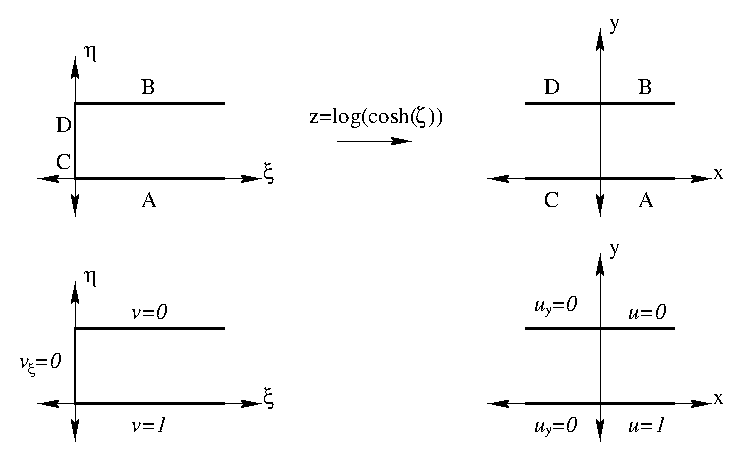
\includegraphics[width=0.8\textwidth]{pde/conformal/sis2is}
    \end{center}
    \caption{The mapping of the boundary conditions.}
    \label{sis2is}
  \end{figure}

  In the $\zeta$ plane, the problem is,
  \begin{gather*}
    v_{\xi\xi} + v_{\eta\eta} = 0, \quad \xi > 0, \quad 0 < \eta < \pi, \\
    v_\xi(0, \eta) = 0, \quad v(\xi, 0) = 1, \quad v(\xi, \pi) = 0.
  \end{gather*}
  By inspection, we see that the solution of this problem is,
  \[
  \boxed{
    v(\xi,\eta) = 1 - \frac{\eta}{\pi}.
    }
  \]
  The solution in the $z$ plane is
  \[
  u(x,y) = 1 - \frac{1}{\pi} \Im \left( \cosh^{-1} (\e^z) \right),
  \]
  where $z = x + \imath y$.  We will find the imaginary part of 
  $\cosh^{-1}(\e^z)$ in order to write this explicitly in terms of $x$ and $y$.
  Recall that we can write the $\cosh^{-1}$ in terms of the logarithm.
  \begin{align*}
    \cosh^{-1}(w) &= \log \left( w + \sqrt{ w^2 - 1 } \right) \\
    \cosh^{-1}(\e^z) &= \log \left( \e^z + \sqrt{ \e^{2z} - 1 } \right) \\
    &= \log \left( \e^z \left( 1 + \sqrt{ 1 - \e^{-2z} } \right) \right) \\
    &= z + \log \left( 1 + \sqrt{ 1 - \e^{-2z} } \right) 
  \end{align*}
  Now we need to find the imaginary part.  We'll work from the inside out.
  First recall,
  \[
  \sqrt{x + \imath y} = \sqrt{ \sqrt{x^2 + y^2} \exp \left( \imath \tan^{-1} 
      \left( \frac{y}{x} \right) \right) }
  = \sqrt[4]{ x^2 + y^2 } \exp \left( \frac{\imath}{2} \tan^{-1}
    \left( \frac{y}{x} \right) \right),
  \]
  so that we can write the innermost factor as,
  \begin{align*}
    \sqrt{1 - \e^{-2 z} }
    &= \sqrt{ 1 - \e^{-2 x} \cos(2 y) + \imath \e^{-2 x} \sin(2 y) } \\
    &= \sqrt[4]{ (1 - \e^{-2 x} \cos(2 y))^2 + (\e^{-2 x} \sin(2 y))^2 }
    \exp \left( \frac{\imath}{2} \tan^{-1} \left(
        \frac{ \e^{-2 x} \sin(2 y) }{ 1 - \e^{-2 x} \cos(2 y) } \right)
    \right) \\
    &= \sqrt[4]{ 1 - 2 \e^{-2 x} \cos(2 y) + \e^{-4 x} }
    \exp \left( \frac{\imath}{2} \tan^{-1} \left(
        \frac{ \sin(2 y) }{ \e^{2x} - \cos(2 y) } \right) \right) 
  \end{align*}
  We substitute this into the logarithm.
  \[
  \log \left( 1 + \sqrt{ 1 - \e^{-2 z} } \right) = 
  \log \left( 1 + \sqrt[4]{ 1 - 2 \e^{-2 x} \cos(2 y) + \e^{-4 x} }
    \exp \left( \frac{\imath}{2} \tan^{-1} \left(
        \frac{ \sin(2 y) }{ \e^{2x} - \cos(2 y) } \right) \right) \right)
  \]
  Now we can write $\eta$.
  \begin{gather*}
    \eta = \Im \left( z + \log \left( 1 + \sqrt{ 1 - \e^{-2 z} } \right) \right) \\
    \eta = y + \tan^{-1} \left(
      \frac{ \sqrt[4]{ 1 - 2 \e^{-2 x} \cos(2 y) + \e^{-4 x} }
        \sin \left( \frac{1}{2} \tan^{-1} \left( 
            \frac{ \sin(2 y) }{ \e^{2x} - \cos(2y) } \right) \right) }
      { 1 + \sqrt[4]{ 1 - 2 \e^{-2 x} \cos(2 y) + \e^{-4 x} }
        \cos \left( \frac{1}{2} \tan^{-1} \left( 
            \frac{ \sin(2 y) }{ \e^{2x} - \cos(2y) } \right) \right) } \right)
  \end{gather*}
  Finally we have the solution, $u(x,y)$.
  \[
  \boxed{
    u(x,y) = 1 - \frac{y}{\pi} - \frac{1}{\pi} \tan^{-1} \left(
      \frac{ \sqrt[4]{ 1 - 2 \e^{-2 x} \cos(2 y) + \e^{-4 x} }
        \sin \left( \frac{1}{2} \tan^{-1} \left( 
            \frac{ \sin(2 y) }{ \e^{2x} - \cos(2y) } \right) \right) }
      { 1 + \sqrt[4]{ 1 - 2 \e^{-2 x} \cos(2 y) + \e^{-4 x} }
        \cos \left( \frac{1}{2} \tan^{-1} \left( 
            \frac{ \sin(2 y) }{ \e^{2x} - \cos(2y) } \right) \right) } \right)
    }
  \]
\end{Solution}









\raggedbottom
}
